% Drawing 70/06-1 -- folder 70, batch 06, archive page 103 (PDF page 104).
% Transcription: petit croquis biffé : $T$, $S$, $\Omega$ reliés par des traits.
% Kind: square of T, S, Omega (fibre product). Method 2 (schematic redraw from the facsimile). Status: ok.
% Notes: Upside down on the page (the page is written tete-beche; crop rotated). T --- T x_S Omega on top, an arrow T -> S down the left, an arrow Omega -> S along the bottom (pointing left), and a short stroke from T x_S Omega down to Omega. Struck out: a blotted sign before the bottom Omega, drawn as a grey struck patch. The transcription calls the whole sketch struck; on the crop only that sign is struck. Redrawn 2026-11-09 (issue 128) after Michel's check: vertices placed once and every edge drawn between them, so concurrent lines meet exactly; labels at \small.
% Coordinates: 1 unit = 1 mm = 1/100 of the crop width (bbox in page fractions: [0.63, 0.7, 0.82, 0.8]).
% Redrawn by Claude (claude-opus-5-5), issue #73, 2026-11-09; not checked by a human; not compiled (no TeX in the session).
% Rights: reproduces part of the work -- behind RENDER_TRANSCRIPTS, never published by itself.
\documentclass[tikz,border=3pt]{standalone}
\usepackage{amsmath,amssymb}
\usetikzlibrary{patterns,arrows.meta}
\tikzset{pencil/.style={black!45}, struck/.style={black!35}, mark/.style={circle,draw,inner sep=1.3pt}, pt/.style={circle,fill,inner sep=0.9pt}, opt/.style={circle,draw,fill=white,inner sep=1.1pt}}
\begin{document}
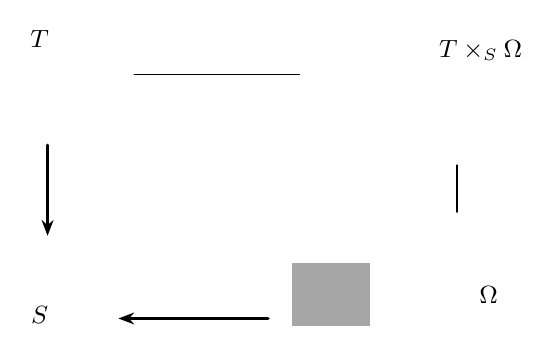
\begin{tikzpicture}[x=1mm,y=1mm,line cap=round,line join=round,font=\scriptsize]
\draw (33,-24) -- (54,-24);
\draw[-{Stealth[length=2mm]},very thick] (22,-33) -- (22,-44.5);
\draw[-{Stealth[length=2mm]},very thick] (50,-55) -- (31,-55);
\draw (74,-35.5) -- (74,-41.5);
\node[inner sep=1pt] at (21,-19.5) {\small $T$};
\node[inner sep=1pt] at (77,-21) {\small $T\times_S\Omega$};
\node[inner sep=1pt] at (21,-54.5) {\small $S$};
\node[inner sep=1pt] at (78,-52) {\small $\Omega$};
\fill[pattern=north east lines,struck] (53,-48) -- (63,-48) -- (63,-56) -- (53,-56) -- cycle;
\end{tikzpicture}
\end{document}
